\documentclass[10pt,conference]{IEEEtran}
\IEEEoverridecommandlockouts
\usepackage{cite}
\usepackage{amsmath,amssymb}
\usepackage{graphicx}
\usepackage{booktabs}
\usepackage{url}
\usepackage[table]{xcolor}
\usepackage{balance}
\usepackage[hidelinks]{hyperref}

% Every inline number comes from tables/macros.tex, generated from data by
% experiments/v2/make_tables_round2.py. No numerical result is typed by hand.
\newcommand{\FONeminDis}{0.001}
\newcommand{\FONemaxDis}{0.096}
\newcommand{\DirectionalityMax}{0.99}
\newcommand{\DirectionalityMin}{0.13}
\newcommand{\FlipRateAllPct}{74.7}
\newcommand{\FlipRateInclUnmitPct}{74.7}
\newcommand{\NearTiePct}{53.3}
\newcommand{\WinnerScope}{the three mitigated methods}
\newcommand{\SplitRegretDefective}{0.0226}
\newcommand{\SplitRegretCorrected}{0.0159}
\newcommand{\SplitRegretExcess}{0.0067}
\newcommand{\PerInstChanged}{11}
\newcommand{\PerInstTotal}{12}
\newcommand{\BudgetMaxDev}{0.0000}
\newcommand{\CollisionCount}{0}
\newcommand{\NumCellsR}{5,040}
\newcommand{\TotalShotsR}{30,240,000}
\newcommand{\CoreHoursR}{1.63}


\newcommand{\code}[1]{\texttt{\small #1}}

\hypersetup{
  pdftitle={Sampling-Free Oracles for Integration Defects in Quantum Error-Mitigation Pipelines},
  pdfauthor={Tran Thi Toi},
  pdfsubject={Quantum error mitigation; software validation},
  pdfkeywords={quantum error mitigation; zero-noise extrapolation; readout error mitigation; validation},
  pdfcreator={},
  pdfproducer={}
}


\begin{document}

\title{Sampling-Free Oracles for Integration Defects\\
in Quantum Error-Mitigation Pipelines}

\author{\IEEEauthorblockN{Tran Thi Toi}
\IEEEauthorblockA{Military Science Academy\\
Hanoi, Vietnam\\
toitt2001@gmail.com}}

\maketitle

\begin{abstract}
Quantum error-mitigation benchmarks are software, and an integration error in the pipeline can move
their conclusions without producing any error or visibly implausible output. We report a bounded
case study of two such errors in a budget-matched zero-noise-extrapolation (ZNE) and readout-error-%
mitigation (REM) pipeline: unitary folding that rebuilds a transpiled circuit's terminal measurements
can discard the layout-induced qubit-to-clbit map, and readout calibration indexed by virtual rather
than physical qubits inverts the response matrix against the wrong qubits. Neither hazard is new --
the standard readout-mitigation library provides \code{final\_measurement\_mapping} for precisely
this purpose, and calibrating the measured physical qubits is documented practice. Our contribution
is a reusable validation artifact and a measurement of consequences. We give \emph{two} deterministic,
sampling-free oracles, and show they are not interchangeable: the folding oracle
($UU^{\dagger}U=U$ must leave the ideal distribution unchanged) is provably blind to the calibration
defect, because at zero readout noise every response matrix is the identity. On a QAOA MaxCut
benchmark over six fixed instances and two device calibration snapshots, run from a fresh seed
namespace with paired common random numbers, the defective and corrected implementations differ by
\FONeminDis--\FONemaxDis{} of $C_{\max}$ depending on the arm (one arm is unaffected), and the
method selected as best changes in \FlipRateAllPct\% of cells among \WinnerScope. That rate
overstates the substantive effect: \TiePracticalAllPct\% of cells are practical near ties. Our
primary endpoint is the paired held-out loss difference between the legacy-selected and
corrected-selected method, measured on an independent evaluation replicate:
\HeldOutDelta{} of $C_{\max}$ (95\% CI [\HeldOutLo, \HeldOutHi]) --- small in absolute terms. We verify
against the standard library used as documented: it agrees with our corrected implementation
exactly, and we make no claim that any released library is defective. All results are
simulator-only and we make no claim of quantum advantage.
\end{abstract}

\begin{IEEEkeywords}
quantum error mitigation, zero-noise extrapolation, readout error mitigation, software correctness,
validation, reproducibility, QAOA
\end{IEEEkeywords}

\section{Introduction}
Comparative benchmarks now guide error-mitigation practice~\cite{cai2023review,bultrini2023,russo2023}.
Those benchmarks are programs, and their conclusions depend on whether the pipeline that implements
the method does what its description says. This paper is a bounded case study of two integration
errors that do not announce themselves, together with the oracles that catch them and a measurement
of how far they can move a benchmark's conclusions.

Once a circuit is transpiled to a device coupling map, the transpiler chooses a layout $\pi$, so
classical bit $c$ records physical qubit $q_{\pi(c)}$. Two things can then go wrong. First, folding
that strips the terminal measurements and rebuilds them with a generic ``measure all'' operation
reinstates $c\leftarrow q_c$ and discards $\pi$. Second, readout calibration indexed by virtual qubit
inverts the response matrix against the wrong qubits.

\subsection*{What is and is not claimed}
\textbf{Neither hazard is a discovery.} Calibrating the physical qubits a circuit actually measures
is documented practice, and \code{mthree} supplies \code{final\_measurement\_mapping} to recover that
map from a transpiled circuit~\cite{nation2021}. We treat this as established, and our positive
control (Section~\ref{sec:control}) shows the library used as documented is unaffected.

We also claim none of the following, all established: that folding leaves state-preparation
and measurement error unamplified~\cite{majumdar2023}; that odd integer scale factors avoid partial
folds~\cite{majumdar2023}; that circuits should be transpiled before amplification~\cite{majumdar2023};
that shot budget governs which method wins~\cite{bultrini2023}; that accuracy gains need not improve
downstream decisions~\cite{scavino2026decision}; or that ZNE can show spurious apparent
improvement~\cite{koester2026}.

\subsection*{Contributions}
\begin{itemize}
\item \textbf{Two sampling-free oracles, and a proof they are not interchangeable.} The folding
      oracle is blind to the calibration defect at zero readout noise; a second oracle with unequal
      response matrices is required. Both are deterministic and need no noise model
      (Section~\ref{sec:oracles}).
\item \textbf{A measurement of consequences} on a complete budget-matched benchmark, with
      instance-level inference and split-sample decision regret (Section~\ref{sec:impact}).
\item \textbf{A positive control} against an independent, correctly used implementation
      (Section~\ref{sec:control}).
\end{itemize}

\section{Background and related work}\label{sec:related}
ZNE estimates the noiseless expectation value by amplifying noise and extrapolating to
zero~\cite{temme2017,li2017}; digital unitary folding implements the amplification by inserting
$U^{\dagger}U$ pairs~\cite{giurgicatiron2020}, as provided by Mitiq~\cite{larose2022mitiq}. Majumdar
\emph{et al.}~\cite{majumdar2023} set out best practices for digital ZNE --- transpile before
amplifying, prefer odd integer scale factors, and compose with readout mitigation because folding
does not amplify SPAM error. We adopt all three as premises.

Readout error is often dominant for shallow circuits~\cite{bravyi2021} and is corrected by inverting
a measured response matrix~\cite{bravyi2021,nation2021}. We use one variant, tensored per-qubit
inversion with clipping; results do not characterise other readout-mitigation methods.

UNITED~\cite{bultrini2023} benchmarks ZNE, Clifford-data regression and virtual distillation against
total shots on random circuits and QAOA MaxCut; readout mitigation is not a compared arm.
Köster and Mauerer~\cite{koester2026} show Richardson ZNE can produce \emph{artefactual} improvement
once amplification pushes the signal below the noise floor --- a \emph{statistical-regime} phenomenon
that occurs in a correct implementation. The errors we study are \emph{integration} errors; they are
independent of that regime and are fixed in code. Sampling-cost bounds~\cite{takagi2022,quek2024}
make cost-equalised comparison the meaningful one.

\section{Problem setting}\label{sec:setting}
\textbf{Task.} QAOA~\cite{farhi2014qaoa} at $p=1$ for MaxCut on six fixed, pairwise non-isomorphic
six-vertex graphs (Table~\ref{tab:instances}). For $G=(V,E)$ the objective is
$C(z)=\sum_{(i,j)\in E}\tfrac12(1-z_iz_j)$. With $|V|=6$ both the exact optimum $C_{\max}$ and the
exact noiseless ansatz value are computable, so ``error'' is unambiguous. The ansatz reference is a
multistart numerical best-known value over 60 exact restarts, \textbf{not} a proven global optimum,
and is labelled as such in the released configuration.

\textbf{Quantities kept distinct.} We separate (i) the difference between two \emph{estimates};
(ii) the difference between two \emph{absolute estimation errors}; (iii) estimator \emph{bias}, the
mean signed deviation from the exact value; and (iv) sampling \emph{variance} across seeds. These
are reported separately and never used interchangeably.

\textbf{Noise.} Two static IBM calibration snapshots: \code{dev\_lagos} (median readout error
$0.169$) and \code{dev\_algiers} ($0.011$). Both \code{cx}-native, holding the folding primitive
fixed. Simulated with Qiskit Aer~\cite{javadiabhari2024qiskit}; \textbf{no quantum hardware was used}.

\textbf{Budget matching.} Each estimate receives the same total shots $B$: the unmitigated arm spends
$B$ on one circuit, ZNE $B/3$ at each of scale factors $(1,3,5)$, REM $0.8B$ on the circuit and
$0.2B$ on $2k$ calibration circuits. Realised totals are asserted per cell; the maximum relative
deviation observed was \BudgetMaxDev\%.

\textbf{Randomness and pairing.} All streams derive from a named coordinate hierarchy. The
implementation label is \emph{deliberately excluded} from the coordinates, so the defective and
corrected runs see identical shot noise for the same cell --- common random numbers, which is what
makes the implementation contrast a within-cell comparison. Every other factor is a coordinate, so
draws are independent across instance, noise, method, budget, seed, basis, scale and replicate. A
collision audit over the realised coordinate set reports \CollisionCount{} collisions; we do not
claim collisions are impossible.

\textbf{Compilation is shared, not drawn per arm.} The transpiler stream depends only on instance,
noise, seed and compilation replicate, so a single prepared base circuit --- same initial layout,
routing permutation and measurement map --- serves every method and implementation within a cell.
Each row carries a fingerprint of that base circuit and the analysis asserts it is identical across
all arms: \CompilationViolations{} violations over \CompilationCellsChecked{} cells. Compilation
and sampling use separate named streams.

\begin{table}[t]
\caption{MaxCut instances. ``best $\langle C\rangle$'' is a multistart numerical best-known value,
\textbf{not} a proven global ansatz optimum; ``at best'' is the fraction of 60 restarts reaching it.}
\label{tab:instances}
\centering\small
\begin{tabular}{@{}lrrrrr@{}}
\toprule
Instance & $|E|$ & $C_{\max}$ & best $\langle C\rangle$ & ratio & at best\\
\midrule
\texttt{prism} & 9 & 7 & 5.9392 & 0.8485 & 95\%\\
\texttt{cycle6} & 6 & 6 & 4.5000 & 0.7500 & 100\%\\
\texttt{k33} & 9 & 9 & 6.2321 & 0.6925 & 97\%\\
\texttt{octahedron} & 12 & 8 & 7.3002 & 0.9125 & 100\%\\
\texttt{path6} & 5 & 5 & 3.8679 & 0.7736 & 52\%\\
\texttt{wheel5} & 10 & 8 & 6.3486 & 0.7936 & 48\%\\
\bottomrule
\end{tabular}

\end{table}

\section{The two defects and their oracles}\label{sec:oracles}

\begin{figure*}[t]
\centering
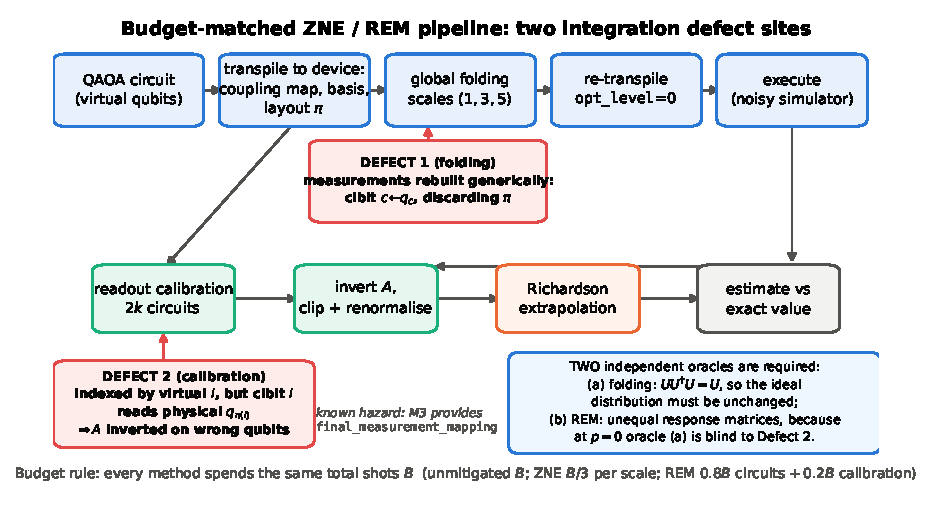
\includegraphics[width=0.90\textwidth]{../figures/fig0_pipeline}
\caption{The budget-matched ZNE/REM pipeline and the two integration defect sites. Both are silent.
Two independent oracles are required, because the folding oracle is blind to the calibration defect
at zero readout noise.}
\label{fig:pipeline}
\end{figure*}

\subsection{Oracle A: folding must preserve the ideal distribution}
Global folding at odd scale $2k{+}1$ implements $U(U^{\dagger}U)^{k}=U$, so the \emph{ideal} output
distribution must be identical to the unfolded circuit's. Any difference is a defect, and no noise
model is needed. On a four-qubit circuit whose ideal outcome is the single bitstring \code{0101}:

\begin{center}\small
\begin{tabular}{@{}lll@{}}
\toprule
\code{initial\_layout} & defective, scale 3 & correct \\
\midrule
\code{[0,1,2,3]} & \code{0101} & \code{0101} \\
\code{[3,2,1,0]} & \code{1010} & \code{0101} \\
\code{[1,3,0,2]} & \code{0011} & \code{0101} \\
\code{[2,0,3,1]} & \code{1100} & \code{0101} \\
\bottomrule
\end{tabular}
\end{center}

\noindent The identity layout hides the defect, which is why it survives casual testing. Comparisons
are made on \emph{exact probability vectors}, not sampled estimates. For Clifford circuits the
agreement is exact to the last bit; with continuous rotations a constant $1.04\times10^{-11}$ offset
appears from floating-point angle representation in the inverted gates --- measured constant at
scales 3, 5 and 9, so it is not length-dependent accumulation, and it is nine orders of magnitude
below the smallest effect reported here.

\subsection{Oracle B: calibration must be checked with unequal response matrices}
\textbf{Oracle A cannot detect the calibration defect.} It runs at zero readout noise, where every
per-qubit response matrix is the identity and any permutation of identities is the identity. We
assert this blindness as a test, so the limitation is recorded rather than assumed.

Oracle B uses deliberately unequal response matrices ($p = 0.30, 0.02, 0.15, 0.05$), a non-identity
measurement map, and an independently computed reference: exact statevector probabilities propagated
through the explicit response matrix. Aligned calibration recovers the ideal distribution to
$\sim\!10^{-16}$; virtual-index calibration fails by up to $1.8\times10^{-1}$
(Table~\ref{tab:oracleB}).

\begin{table}[t]
\caption{Oracle B. Maximum absolute error in the recovered distribution. The identity layout is a
degenerate case in which the defect is invisible.}
\label{tab:oracleB}
\centering\small
\begin{tabular}{@{}lrr@{}}
\toprule
\code{initial\_layout} & aligned calibration & virtual-index calibration \\
\midrule
\code{[0,1,2,3]} & $1.1\times10^{-16}$ & $1.1\times10^{-16}$ \\
\code{[3,2,1,0]} & $5.6\times10^{-17}$ & $1.8\times10^{-1}$ \\
\code{[1,3,0,2]} & $5.6\times10^{-17}$ & $1.3\times10^{-1}$ \\
\code{[2,0,3,1]} & $1.7\times10^{-16}$ & $4.9\times10^{-2}$ \\
\bottomrule
\end{tabular}
\end{table}

\subsection{When the defects are invisible}
Neither defect is detectable in all circumstances, and we state the conditions rather than claim
universality. A non-identity permutation is invisible whenever the state and observable are symmetric
under it. Calibration misindexing is invisible whenever the per-qubit response matrices are equal,
which includes every zero-readout-noise case.

\subsection{What folding amplifies}
Computing exact density-matrix probabilities and applying the readout response matrix explicitly,
$p_{\text{meas}}=A\,p$: under gate noise alone $\langle ZZ\rangle$ falls from $0.9801$ to $0.9044$
between scales 1 and 5, whereas under readout noise alone it is $0.8100$ at every scale --- exactly
$(1-2p)^2$ for $p=0.05$. Readout error therefore contributes a \emph{constant attenuation that does
not vary with the scale factor}, so folding cannot extrapolate it away. This confirms rather than
discovers the point in~\cite{majumdar2023}.

\section{Positive control against an independent implementation}\label{sec:control}
We run \code{mthree}~\cite{nation2021} as documented, recovering the measurement map with
\code{final\_measurement\_mapping}. Its independently implemented map agrees with ours on every
layout tested, and both recover the exact distribution to machine precision; only the virtual-index
integration fails. \textbf{We do not misuse a library and then call it defective}: the contrast is
between a correct integration and an incorrect one. Details in the supplementary material.

\section{Consequences on a benchmark}\label{sec:impact}
Identical configurations --- same instances, noise, budget, seeds --- were run through the defective
and corrected implementations under common random numbers, from a fresh seed namespace, with the
SHA-256 content hash of every execution-path file recorded per row. Differences are normalised by
each instance's own $C_{\max}$ before averaging.

\textbf{Inference scope.} Primary inference is over the \textbf{six fixed instances}, with
uncertainty from a stratified bootstrap resampling seeds within each instance. A secondary
instance-level cluster bootstrap (6 clusters) indicates what generalisation beyond these instances
would look like; it is always wider and is reported alongside.

\begin{table*}[t]
\caption{Implementation contrast, paired within cell under common random numbers, normalised by
$C_{\max}$. \emph{Directionality} is $|\text{mean signed}|/\text{mean}|\cdot|$: values near 1 indicate
a one-directional shift, not cancellation. The cluster interval is the weaker generalisation-oriented
interval. $p_{\mathrm{BH}}$ is adjusted within the declared family; BH adjustment does not repair a
sampling model and is applied only after the estimand and dependence structure are fixed.}
\label{tab:f1}
\centering\small
\begin{tabular}{@{}llrrllrrr@{}}
\toprule
Noise & Method & $n$ & mean signed & 95\% CI (stratified) & 95\% CI (cluster) & mean $|\cdot|$ & direct. & $p_{\mathrm{BH}}$\\
\midrule
\texttt{dev\_algiers} & REM & 180 & -0.0002 & [-0.0003, -0.0000] & [-0.0003, -0.0001] & 0.0007 & 0.24 & $0.012$\\
\texttt{dev\_algiers} & ZNE & 180 & +0.0610 & [+0.0583, +0.0636] & [+0.0302, +0.0962] & 0.0619 & 0.98 & $1.5\times10^{-29}$\\
\texttt{dev\_algiers} & ZNE+REM & 180 & +0.0693 & [+0.0665, +0.0720] & [+0.0357, +0.1069] & 0.0702 & 0.99 & $1.4\times10^{-29}$\\
\texttt{dev\_lagos} & REM & 180 & -0.0342 & [-0.0442, -0.0248] & [-0.0465, -0.0229] & 0.0569 & 0.60 & $2.6\times10^{-13}$\\
\texttt{dev\_lagos} & ZNE & 180 & -0.0211 & [-0.0222, -0.0200] & [-0.0348, -0.0101] & 0.0218 & 0.97 & $7.3\times10^{-29}$\\
\texttt{dev\_lagos} & ZNE+REM & 180 & -0.0443 & [-0.0592, -0.0289] & [-0.0632, -0.0241] & 0.0938 & 0.47 & $2.0\times10^{-9}$\\
\bottomrule
\end{tabular}

\end{table*}

\begin{table*}[t]
\caption{Estimator bias and sampling variance, reported \emph{separately} from differences of
absolute errors and normalised by $C_{\max}$. Note that on \code{dev\_algiers} the defective
implementation gives ZNE a large \emph{positive} bias where the corrected one is near zero --- a
one-directional shift, not a symmetric scatter.}
\label{tab:bv}
\centering\small
\begin{tabular}{@{}lllrlrr@{}}
\toprule
Noise & Method & Impl. & bias & 95\% CI & sd & RMSE\\
\midrule
\texttt{dev\_algiers} & unmitigated & v2 & -0.0299 & [-0.0302, -0.0296] & 0.0023 & 0.0301\\
\texttt{dev\_algiers} & REM & legacy & -0.0239 & [-0.0243, -0.0234] & 0.0032 & 0.0242\\
\texttt{dev\_algiers} & REM & v2 & -0.0240 & [-0.0245, -0.0236] & 0.0033 & 0.0244\\
\texttt{dev\_algiers} & ZNE & legacy & +0.0700 & [+0.0678, +0.0723] & 0.0158 & 0.0836\\
\texttt{dev\_algiers} & ZNE & v2 & -0.0070 & [-0.0083, -0.0057] & 0.0088 & 0.0112\\
\texttt{dev\_algiers} & ZNE+REM & legacy & +0.0785 & [+0.0759, +0.0811] & 0.0180 & 0.0924\\
\texttt{dev\_algiers} & ZNE+REM & v2 & -0.0011 & [-0.0027, +0.0006] & 0.0117 & 0.0118\\
\texttt{dev\_lagos} & unmitigated & v2 & -0.1464 & [-0.1469, -0.1459] & 0.0034 & 0.1492\\
\texttt{dev\_lagos} & REM & legacy & -0.0979 & [-0.1055, -0.0906] & 0.0530 & 0.1129\\
\texttt{dev\_lagos} & REM & v2 & -0.1321 & [-0.1400, -0.1258] & 0.0511 & 0.1430\\
\texttt{dev\_lagos} & ZNE & legacy & -0.1082 & [-0.1097, -0.1067] & 0.0105 & 0.1099\\
\texttt{dev\_lagos} & ZNE & v2 & -0.1293 & [-0.1309, -0.1278] & 0.0107 & 0.1333\\
\texttt{dev\_lagos} & ZNE+REM & legacy & -0.0714 & [-0.0857, -0.0577] & 0.0985 & 0.1261\\
\texttt{dev\_lagos} & ZNE+REM & v2 & -0.1314 & [-0.1387, -0.1238] & 0.0520 & 0.1443\\
\bottomrule
\end{tabular}

\end{table*}

Table~\ref{tab:f1} reports the contrast. The shift is \textbf{not} direction-free: directionality
exceeds \DirectionalityMax{} for the largest arms, so the defect moves those estimates
predominantly one way. Table~\ref{tab:bv} separates estimator bias from sampling variance, which
Table~\ref{tab:f1} deliberately does not conflate.

\begin{table*}[t]
\caption{Primary endpoint: the paired held-out loss difference between the method selected under the
defective implementation and the method selected under the corrected one, measured on an
\emph{independent} evaluation replicate and normalised by $C_{\max}$. Positive values mean the
defective selection is worse. The estimand is the mean over the six fixed instances; the stratified
interval resamples seeds within instance and the cluster interval resamples instances. No minimum
over methods is taken, so no noisy per-replicate minimum is treated as a minimum expected risk.}
\label{tab:endpoint}
\centering\small
\begin{tabular}{@{}llrrllr@{}}
\toprule
Candidate set & Noise & $n$ & $\Delta_{\text{held-out}}$ & 95\% CI (stratified) & 95\% CI (cluster) & winner changed\\
\midrule
mitigated only & \texttt{dev\_algiers} & 180 & +0.0019 & [+0.0017, +0.0021] & [+0.0013, +0.0024] & 92.8\% \\
mitigated only & \texttt{dev\_lagos} & 180 & -0.0005 & [-0.0016, +0.0006] & [-0.0014, +0.0005] & 60.0\% \\
mitigated only & all & 360 & +0.0007 & [+0.0001, +0.0013] & [+0.0003, +0.0011] & 76.4\% \\
incl.\ unmitigated & \texttt{dev\_algiers} & 180 & +0.0020 & [+0.0018, +0.0021] & [+0.0014, +0.0024] & 92.8\% \\
incl.\ unmitigated & \texttt{dev\_lagos} & 180 & -0.0005 & [-0.0016, +0.0006] & [-0.0014, +0.0005] & 60.0\% \\
incl.\ unmitigated & all & 360 & +0.0007 & [+0.0001, +0.0013] & [+0.0004, +0.0012] & 76.4\% \\
\bottomrule
\end{tabular}

\end{table*}

\begin{table*}[t]
\caption{Near ties, reported separately for all cells and for changed-winner cells, and for each
candidate set. The gap is between the best and second-best candidate on the \emph{selection}
replicate under the corrected implementation --- the view a correctly implemented benchmark would
have when choosing. \emph{Practical} means that gap is below the declared threshold
$0.01\,C_{\max}$; \emph{statistical} means it is within the Monte-Carlo scale of the selection
replicate. These are different notions and are not merged.}
\label{tab:ties}
\centering\small
\begin{tabular}{@{}llrrrrrr@{}}
\toprule
 & & & \multicolumn{2}{c}{practical ($<0.01\,C_{\max}$)} & \multicolumn{2}{c}{statistical} & \\
\cmidrule(lr){4-5}\cmidrule(lr){6-7}
Candidate set & Noise & $n$ & all & changed & all & changed & median gap\\
\midrule
mitigated only & \texttt{dev\_algiers} & 180 & 100.0\% & 100.0\% & 100.0\% & 100.0\% & 0.0008\\
mitigated only & \texttt{dev\_lagos} & 180 & 91.7\% & 92.6\% & 100.0\% & 100.0\% & 0.0033\\
mitigated only & all & 360 & 95.8\% & 97.1\% & 100.0\% & 100.0\% & 0.0015\\
incl.\ unmitigated & \texttt{dev\_algiers} & 180 & 100.0\% & 100.0\% & 100.0\% & 100.0\% & 0.0008\\
incl.\ unmitigated & \texttt{dev\_lagos} & 180 & 92.8\% & 94.4\% & 100.0\% & 100.0\% & 0.0032\\
incl.\ unmitigated & all & 360 & 96.4\% & 97.8\% & 100.0\% & 100.0\% & 0.0014\\
\bottomrule
\end{tabular}

\end{table*}

\begin{figure*}[t]
\centering
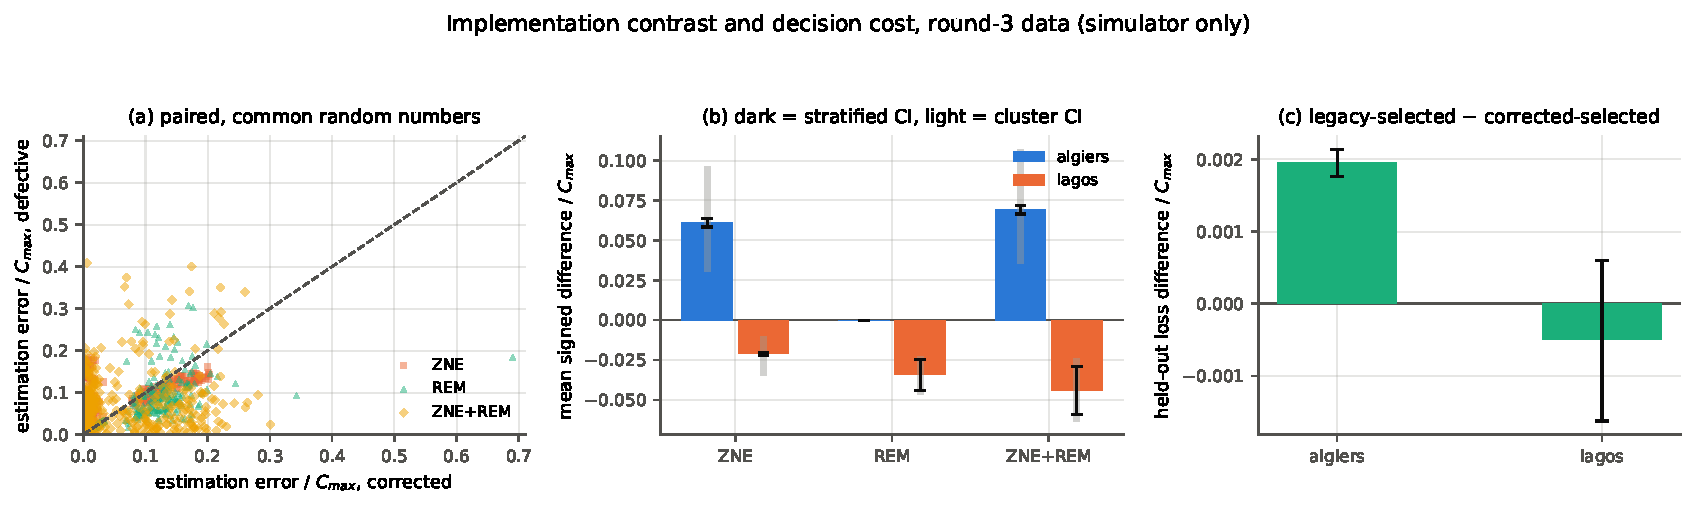
\includegraphics[width=\textwidth]{../figures/figR3_impact}
\caption{Implementation contrast and decision cost on the round-3 data. (a) Per-cell estimation error,
defective versus corrected, paired under common random numbers. (b) Mean normalised difference with
stratified (solid) and cluster (light) intervals. (c) Paired held-out loss difference between the two selections. Simulator only.}
\label{fig:impact}
\end{figure*}

\textbf{Decision cost, measured out of sample.} Table~\ref{tab:endpoint} reports the primary
endpoint. Table~\ref{tab:ties} reports near ties along two separate axes --- practical and
statistical --- for all cells and for changed-winner cells, and for both candidate sets. A
substantial share of cells are near ties, so a changed winner does not by itself imply a substantive
ranking change. That is precisely why the endpoint is a paired held-out difference between two named
selections rather than a gap to a same-sample minimum; we do not describe any same-sample minimum as
``best attainable''.

\begin{figure*}[t]
\centering
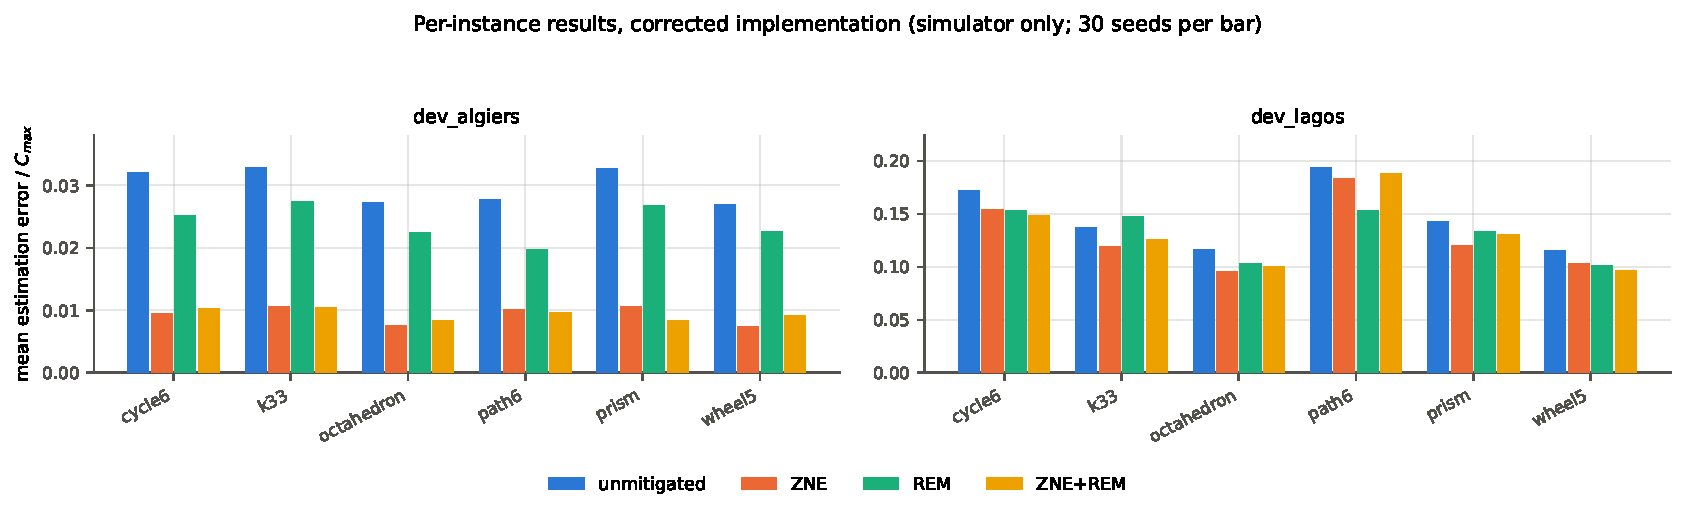
\includegraphics[width=\textwidth]{../figures/figR3_perinstance}
\caption{Per-instance results. Pooled means conceal instance-to-instance heterogeneity, which is why
inference is instance-aware. Simulator only.}
\label{fig:perinst}
\end{figure*}

\section{A pilot correction}\label{sec:pilot}
This work began as a correction to our own unpublished pilot. In that pilot the transpiler chose
non-identity layouts for three of twelve conditions, so the mitigated arms there used defective code:
$450$ of $2400$ estimation cells and $30$ of $40$ optimisation runs. A conclusion the pilot had drawn
about in-loop optimisation rested entirely on affected runs and is not carried forward; this paper
makes no in-loop claim. We also found, and report, that the pilot's own ``confirmation'' run was not
independent: its seed coordinates omitted the instance, noise, method and budget, so all 224 of its
rows reproduced main-study values bit-for-bit. That pilot data is retained as a single exploratory
campaign and no confirmatory claim rests on it. We record this because it is the reason the oracles
in Section~\ref{sec:oracles} exist, not as a contribution.

\section{Threats to validity}\label{sec:threats}
\textbf{Simulator only.} Aer snapshots omit crosstalk, drift, leakage and non-Markovian effects.
\textbf{Scope.} Six fixed instances, $p=1$, six qubits; instances are not a random sample and
generalisation beyond them is indicated only by the wider cluster interval.
\textbf{Single implementations.} Global folding, Richardson extrapolation, tensored inversion with
clipping; results do not characterise other readout-mitigation methods or local folding.
\textbf{Device family.} IBM \code{cx}-native snapshots only.
\textbf{Generality of the defects.} Demonstrated in one pipeline built on widely used components.
We have not audited third-party libraries, and the positive control indicates the standard library
used as documented is unaffected.
\textbf{Dependence.} Seeds are nested within instance and recur across arms; observations are not
independent draws and are not analysed as such.
\textbf{Round-1 data} was generated with correlated streams and a dirty working tree; it is reported
as exploratory, its provenance is reconstructed rather than relabelled, and no claim rests on it.

\section{Reproducibility and data availability}\label{sec:repro}
Code, protocols, configurations, raw per-cell records, processed results, figure sources and the
regression tests accompany this submission with a pinned environment. Every number is generated from
raw data by the analysis scripts; none is transcribed by hand, and a traceability table maps each
quantitative claim to a file, configuration, command and output table. Round-2 rows record the
SHA-256 content hash of every execution-path file. The repository is currently private and will be
made public on acceptance; we do not claim public availability before then.

\section{Conclusion}
Two integration errors in an error-mitigation pipeline changed which method a benchmark selected,
without producing any error or implausible output. Neither hazard is new, and the standard tooling
already solves one of them. What we offer is a pair of deterministic, sampling-free oracles --- and
the observation that they are not interchangeable, since the folding oracle is provably blind to the
calibration defect --- together with a measurement of how far such an error can move a complete
benchmark. We recommend asserting the measurement map after any circuit rewrite, and indexing
readout calibration by the physical qubits the classical bits actually read.

\balance
\bibliographystyle{IEEEtran}
\bibliography{references}

\end{document}
